\documentclass{article}
\usepackage{tikz}
\usetikzlibrary{positioning}

\begin{document}

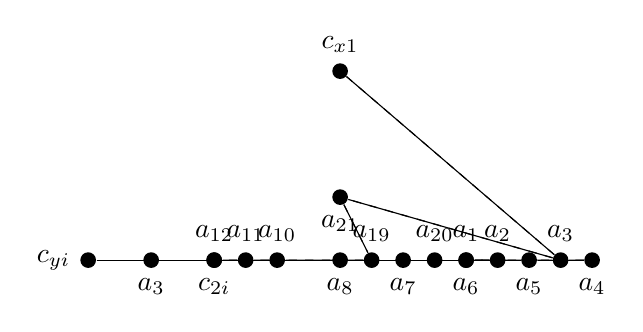
\begin{tikzpicture}[scale=0.8]
    % Define coordinates for the vertices
    \node[circle,fill,inner sep=2pt,label=left:$c_{yi}$] (c1) at (-4,-1) {};
    \node[circle,fill,inner sep=2pt,label=below:$c_{2i}$] (c2) at (-2,-1) {};
    \node[circle,fill,inner sep=2pt,label=below:$a_8$] (a8) at (0,-1) {};
    \node[circle,fill,inner sep=2pt,label=below:$a_7$] (a7) at (1,-1) {};
    \node[circle,fill,inner sep=2pt,label=below:$a_6$] (a6) at (2,-1) {};
    \node[circle,fill,inner sep=2pt,label=below:$a_5$] (a5) at (3,-1) {};
    \node[circle,fill,inner sep=2pt,label=below:$a_4$] (a4) at (4,-1) {};
    \node[circle,fill,inner sep=2pt,label=below:$a_3$] (a3) at (-3,-1) {};
    \node[circle,fill,inner sep=2pt,label=below:$a_{21}$] (a21) at (0,0) {};
    \node[circle,fill,inner sep=2pt,label=above:$a_{19}$] (a19) at (0.5,-1) {};
    \node[circle,fill,inner sep=2pt,label=above:$a_{10}$] (a10) at (-1,-1) {};
    \node[circle,fill,inner sep=2pt,label=above:$a_{11}$] (a11) at (-1.5,-1) {};
    \node[circle,fill,inner sep=2pt,label=above:$a_{12}$] (a12) at (-2,-1) {};
    \node[circle,fill,inner sep=2pt,label=above:$a_{20}$] (a20) at (1.5,-1) {};
    \node[circle,fill,inner sep=2pt,label=above:$a_{2}$] (a2) at (2.5,-1) {};
    \node[circle,fill,inner sep=2pt,label=above:$a_{1}$] (a1) at (2,-1) {};
    \node[circle,fill,inner sep=2pt,label=above:$a_{3}$] (a3) at (3.5,-1) {};
    \node[circle,fill,inner sep=2pt,label=above:$c_{x1}$] (cx1) at (0,2) {};

    % Draw the edges
    \draw[dashed] (c1) -- (a8);
    \draw[dashed] (c2) -- (a7);
    \draw[dashed] (a7) -- (a6);
    \draw[dashed] (a6) -- (a5);
    \draw[dashed] (a5) -- (a4);
    \draw[dashed] (a4) -- (a3);
    \draw[dashed] (a3) -- (a21);
    \draw[dashed] (a21) -- (a19);
    \draw[dashed] (a19) -- (a10);
    \draw[dashed] (a10) -- (a11);
    \draw[dashed] (a11) -- (a12);
    \draw[dashed] (a12) -- (a20);
    \draw[dashed] (a20) -- (a2);
    \draw[dashed] (a2) -- (a1);
    \draw[dashed] (a1) -- (a3);
    \draw[dashed] (a3) -- (cx1);

    % Draw the edges connecting the vertices to the clause gadget
    \draw (c1) -- (a8);
    \draw (c2) -- (a7);
    \draw (a7) -- (a6);
    \draw (a6) -- (a5);
    \draw (a5) -- (a4);
    \draw (a4) -- (a3);
    \draw (a3) -- (a21);
    \draw (a21) -- (a19);
    \draw (a19) -- (a10);
    \draw (a10) -- (a11);
    \draw (a11) -- (a12);
    \draw (a12) -- (a20);
    \draw (a20) -- (a2);
    \draw (a2) -- (a1);
    \draw (a1) -- (a3);
    \draw (a3) -- (cx1);
\end{tikzpicture}

\end{document}